
\documentclass[11pt,fleqn]{article} 
\usepackage[margin=0.8in, head=0.8in]{geometry} 
\usepackage{amsmath, amssymb, amsthm}
\usepackage{fancyhdr} 
\usepackage{palatino, url, multicol}
\usepackage{graphicx, pgfplots,xfrac} 
\usepackage[all]{xy}
\usepackage{polynom} 
%\usepackage{pdfsync} %% I don't know why this messes up tabular column widths
\usepackage{enumerate}
\usepackage{framed}
\usepackage{setspace}
\usepackage{array,tikz}

\pgfplotsset{compat=1.6}

\pgfplotsset{soldot/.style={color=black,only marks,mark=*}} \pgfplotsset{holdot/.style={color=black,fill=white,only marks,mark=*}}


\pagestyle{fancy} 
\lfoot{}
\rfoot{ Midterm I prep}

\begin{document}
\renewcommand{\headrulewidth}{0pt}
\newcommand{\blank}[1]{\rule{#1}{0.75pt}}
\newcommand{\bc}{\begin{center}}
\newcommand{\ec}{\end{center}}
\renewcommand{\d}{\displaystyle}

\vspace*{-0.7in}

%%%%%%%%%intro page
\begin{center}
  \large
  \sc{Recitation: Week 5}\\ \vfill
\end{center}
\vspace*{-.25in}
\begin{enumerate}
\item \textbf{TYPE:} Secant lines and tangent lines.
Let $f(x)=1+ \frac{4}{x}.$
\begin{enumerate}
	\item Find the slope of the secant line between $P(1,f(1)$ and $Q=(2,f(2)).$
	\item Write an equation of the tangent line to the graph of $f(x)$ at $x=2.$
	\item Sketch $f(x)$, the tangent line and the secant line on the same axes.
	\item If $f$ represented position and $x$ represented time, which of the calculations above would be average velocity and which would be instantaneous velocity?
\end{enumerate}

\item  \textbf{TYPE:} Definition of the derivative.
\begin{enumerate}
	\item State the definition of the derivative.
	\item Use the definition of the derivative to find the derivative of $f(x)=\sqrt{3x}.$ No credit will be given for answers not using the definition. Points will be deducted for poorly written answers.
\end{enumerate}

\item \textbf{TYPE:} Derivative as rate of change. 
The  number of bacteria after $t$ hours in a controlled laboratory setting is given by the function $n=f(t)$ where $n$ is the number of bacteria and $t$ is measured in hours.
\begin{enumerate}
	\item Suppose $f'(5)=2000.$ What are the units of the derivative?
	\item In the context of the problem, explain what $f'(5)=2000$ means using complete sentences. 
	\item If $f(5)=40,000,$ how would you estimate $f(7)$ given the available information?
\end{enumerate} 

\item \textbf{TYPE:} Evaluating limits.
Evaluate the limits below. Justify your answer with words and/or algebra.
\begin{multicols}{3}
\begin{enumerate}
	\item$\displaystyle{\lim_{x\to-3 }\frac{x^2+3x}{x^2-x-12}}$
	\item $\displaystyle{\lim_{x\to1^+} \ln\left(\frac{5-x^2}{1+x}\right) }$
	\item $\displaystyle{\lim_{x\to4^-}\frac{\sqrt{x}}{(x-4)^5} }$
	\item $\displaystyle{\lim_{x\to 5}\frac{\frac{1}{x}-\frac{1}{25}}{x-5}}$
	\item $\displaystyle{\lim_{x\to 7}\left(x+\frac{x-7}{\sqrt{x}-\sqrt{7}}\right)}$
\end{enumerate} 
\end{multicols}

\item \textbf{TYPE:} Position, Velocity, Acceleration\\
A particle is moving back and forth along a straight line. The position function of a particle is given by $s(t)=\frac{1}{3}t^3-4t^2+12t$ where $t$ is measured in seconds and $s$ in meters.  
\begin{enumerate}
	\item What is the velocity function of the particle?
	\item What is the acceleration function of the particle?
	\item At $t=3,$ is the particle speeding up or slowing down?
	\item When does the particle turn around?
	\item When is the particle moving to the right?
\end{enumerate} 

\item \textbf{TYPE:} Derivative as Function
\begin{multicols}{2}
Using the graph of $f(x)$ below, sketch the graph of $f'(x).$\\
\includegraphics[scale=.2]{week5-pic}
\end{multicols}

\item \textbf{TYPE:} Derivatives\\
Find the derivatives for each function below. You do not need to simplify but you must use parentheses correctly.
\begin{enumerate}
	\item $g(x)=\frac{2}{x}-3\left(\frac{x^2+1}{5}\right)+2\sqrt{2}$
	\item $h(x)=\cos(x) - \sqrt{x} \sin(x)$
	\item $k(x)= x^2-\frac{x^2+2}{5+\sin(x)}$
\end{enumerate} 

\item \textbf{TYPE:} Graphical Limits\\

For the function $f(x)$ whose graph is given below,
state the value of each quantity if it exists.

\begin{center}
  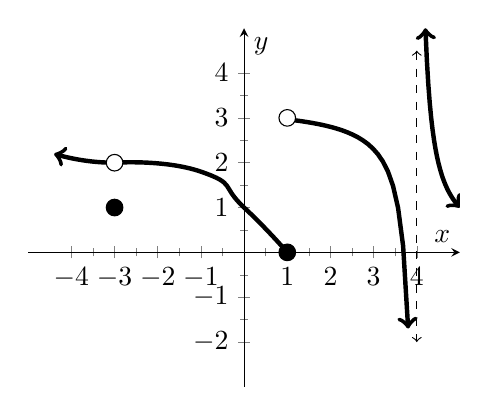
\begin{tikzpicture}
\begin{axis}[scale=.8, axis x line=middle, axis y line=
middle, xlabel={$x$}, ylabel={$y$}, xtick={-4,-3,...,4}, ytick={-2,-1,...,4},
xmin=-5, xmax=5, ymin=-3, ymax=5, minor y tick num=1,
        minor x tick num=1, mark size=3.0pt]
\addplot[domain=-4.4:-3,<-,ultra thick] {0.1*((x+3)^2)+2};
\addplot[domain=-3:1, smooth, tension=1, ultra thick] coordinates { (-3,2) (-1,1.8) (0,1) (1,0)};
\addplot[domain=1:3.8, ultra thick,->] {(x-4)^(-1)+3.3};
\addplot[domain=4.2:5,<->, ultra thick]{(x-4)^(-1)};
\addplot[dashed,<->] coordinates {(4,4.5) (4,-2)};
\addplot[mark=*,only marks] coordinates {(-3,1)(1,0)};
\addplot[mark=*,fill=white,only marks] coordinates {(-3,2)(1,3)};
\end{axis}
\end{tikzpicture}
\end{center}

  \begin{multicols}{3}
\vspace*{-0.5in}
    \begin{enumerate}
    \item $\d \lim_{x \to -3} f(x) =$ \blank{0.5in}
    \item $f(-3) =$ \blank{0.5in}
    \item $\d \lim_{x \to 1^-} f(x) =$ \blank{0.5in}
    \item $\d \lim_{x \to 1^+} f(x) =$ \blank{0.5in}
    \item $\d \lim_{x \to 1} f(x) =$ \blank{0.5in}
    \item $f(1) =$ \blank{0.5in}
    \item $\d \lim_{x \to 4^-} f(x) =$ \blank{0.5in}
    \item $\d \lim_{x \to 4^+} f(x) =$ \blank{0.5in}
    \end{enumerate}
\end{multicols}

\item \textbf{TYPE:} Graphical Contintuity \& Differentiability\\
A graph of the function $f(x)$ is displayed
below. 
\begin{multicols}{2}
\begin{center}
  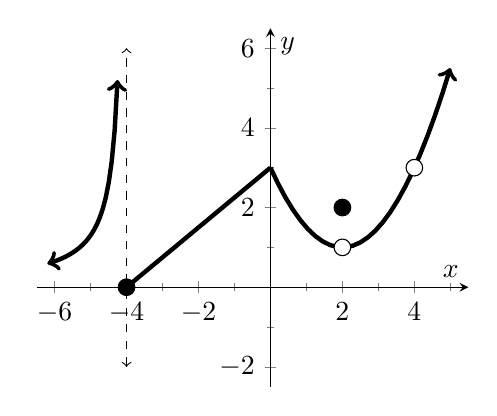
\begin{tikzpicture}
\begin{axis}[scale=.8, axis x line=middle, axis y line=
middle, xlabel={$x$}, ylabel={$y$}, xtick={-6,-4,...,6}, ytick={-2,0,...,6},
xmin=-6.5, xmax=5.5, ymin=-2.5, ymax=6.5, minor y tick num=1,
        minor x tick num=1, mark size=3.0pt]
\addplot[domain=-6.2:-4.25,<->,ultra thick] {1.3*(-4-x)^(-1)};
\addplot[ultra thick] coordinates {(-4,0) (0,3)};
\addplot[domain=0:5,->, ultra thick] {1+0.5*(x-2)^2};
\addplot[dashed,<->] coordinates {(-4,-2) (-4,6)};
\addplot[mark=*,only marks] coordinates {(-4,0) (2,2)};
\addplot[mark=*,fill=white,only marks] coordinates {(2,1)(4,3)};
\end{axis}
\end{tikzpicture}
\end{center}

\begin{enumerate}[(a)]

  \item From the graph of $f$, state the numbers at which
    $f$ is discontinuous and why.
\vfill
  \item From the graph of $f$, state the numbers at which
    $f$ fails to be differentiable and why. 
\vfill
  \end{enumerate}
\end{multicols}

\item \textbf{TYPE:} One and Two Sided Limits\\
Given $f(x) =
  \begin{cases}
  3 & x \ge 4  \\
    \frac{3x - 12}{|x-4|} & x < 4 
  \end{cases}$ find $\d \lim_{x \to 4} f(x)$ or explain why this limit
  does not exist. 
  
 \item \textbf{TYPE:} Intermediate Value Theorem\\
 Using complete sentences, use the Intermediate
Value Theorem to show that there is a root of the equation $e^x = 3 -
2x$ in the interval $(0, 1)$. 
  
\end{enumerate}
\end{document}

\item \textbf{TYPE:} \\
\begin{enumerate}
	\item
\end{enumerate} 
